\documentclass[1p]{elsarticle_modified}
%\bibliographystyle{elsarticle-num}

%\usepackage[colorlinks]{hyperref}
%\usepackage{abbrmath_seonhwa} %\Abb, \Ascr, \Acal ,\Abf, \Afrak
\usepackage{amsfonts}
\usepackage{amssymb}
\usepackage{amsmath}
\usepackage{amsthm}
\usepackage{scalefnt}
\usepackage{amsbsy}
\usepackage{kotex}
\usepackage{caption}
\usepackage{subfig}
\usepackage{color}
\usepackage{graphicx}
\usepackage{xcolor} %% white, black, red, green, blue, cyan, magenta, yellow
\usepackage{float}
\usepackage{setspace}
\usepackage{hyperref}

\usepackage{tikz}
\usetikzlibrary{arrows}

\usepackage{multirow}
\usepackage{array} % fixed length table
\usepackage{hhline}

%%%%%%%%%%%%%%%%%%%%%
\makeatletter
\renewcommand*\env@matrix[1][\arraystretch]{%
	\edef\arraystretch{#1}%
	\hskip -\arraycolsep
	\let\@ifnextchar\new@ifnextchar
	\array{*\c@MaxMatrixCols c}}
\makeatother %https://tex.stackexchange.com/questions/14071/how-can-i-increase-the-line-spacing-in-a-matrix
%%%%%%%%%%%%%%%

\usepackage[normalem]{ulem}

\newcommand{\msout}[1]{\ifmmode\text{\sout{\ensuremath{#1}}}\else\sout{#1}\fi}
%SOURCE: \msout is \stkout macro in https://tex.stackexchange.com/questions/20609/strikeout-in-math-mode

\newcommand{\cancel}[1]{
	\ifmmode
	{\color{red}\msout{#1}}
	\else
	{\color{red}\sout{#1}}
	\fi
}

\newcommand{\add}[1]{
	{\color{blue}\uwave{#1}}
}

\newcommand{\replace}[2]{
	\ifmmode
	{\color{red}\msout{#1}}{\color{blue}\uwave{#2}}
	\else
	{\color{red}\sout{#1}}{\color{blue}\uwave{#2}}
	\fi
}

\newcommand{\Sol}{\mathcal{S}} %segment
\newcommand{\D}{D} %diagram
\newcommand{\A}{\mathcal{A}} %arc


%%%%%%%%%%%%%%%%%%%%%%%%%%%%%5 test

\def\sl{\operatorname{\textup{SL}}(2,\Cbb)}
\def\psl{\operatorname{\textup{PSL}}(2,\Cbb)}
\def\quan{\mkern 1mu \triangleright \mkern 1mu}

\theoremstyle{definition}
\newtheorem{thm}{Theorem}[section]
\newtheorem{prop}[thm]{Proposition}
\newtheorem{lem}[thm]{Lemma}
\newtheorem{ques}[thm]{Question}
\newtheorem{cor}[thm]{Corollary}
\newtheorem{defn}[thm]{Definition}
\newtheorem{exam}[thm]{Example}
\newtheorem{rmk}[thm]{Remark}
\newtheorem{alg}[thm]{Algorithm}

\newcommand{\I}{\sqrt{-1}}
\begin{document}

%\begin{frontmatter}
%
%\title{Boundary parabolic representations of knots up to 8 crossings}
%
%%% Group authors per affiliation:
%\author{Yunhi Cho} 
%\address{Department of Mathematics, University of Seoul, Seoul, Korea}
%\ead{yhcho@uos.ac.kr}
%
%
%\author{Seonhwa Kim} %\fnref{s_kim}}
%\address{Center for Geometry and Physics, Institute for Basic Science, Pohang, 37673, Korea}
%\ead{ryeona17@ibs.re.kr}
%
%\author{Hyuk Kim}
%\address{Department of Mathematical Sciences, Seoul National University, Seoul 08826, Korea}
%\ead{hyukkim@snu.ac.kr}
%
%\author{Seokbeom Yoon}
%\address{Department of Mathematical Sciences, Seoul National University, Seoul, 08826,  Korea}
%\ead{sbyoon15@snu.ac.kr}
%
%\begin{abstract}
%We find all boundary parabolic representation of knots up to 8 crossings.
%
%\end{abstract}
%\begin{keyword}
%    \MSC[2010] 57M25 
%\end{keyword}
%
%\end{frontmatter}

%\linenumbers
%\tableofcontents
%
\newcommand\colored[1]{\textcolor{white}{\rule[-0.35ex]{0.8em}{1.4ex}}\kern-0.8em\color{red} #1}%
%\newcommand\colored[1]{\textcolor{white}{ #1}\kern-2.17ex	\textcolor{white}{ #1}\kern-1.81ex	\textcolor{white}{ #1}\kern-2.15ex\color{red}#1	}

{\Large $\underline{12n_{0465}~(K12n_{0465})}$}

\setlength{\tabcolsep}{10pt}
\renewcommand{\arraystretch}{1.6}
\vspace{1cm}\begin{tabular}{m{100pt}>{\centering\arraybackslash}m{274pt}}
\multirow{5}{120pt}{
	\centering
	\includegraphics[width=112pt]{../../../GIT/diagram.site/Diagrams/png/2554_12n_0465.png}\\
\ \ \ A knot diagram\footnotemark}&
\allowdisplaybreaks
\textbf{Linearized knot diagam} \\
\cline{2-2}
 &
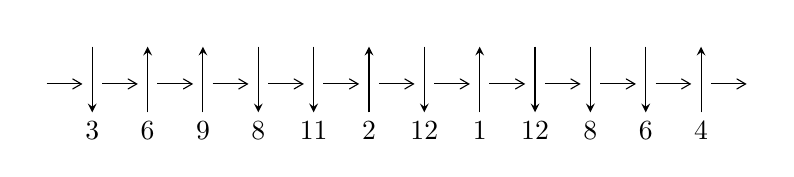
\begin{tikzpicture}[x=20pt, y=17pt]
	% nodes
	\node (C0) at (0, 0) {};
	\node (C1) at (1, 0) {};
	\node (C1U) at (1, +1) {};
	\node (C1D) at (1, -1) {3};

	\node (C2) at (2, 0) {};
	\node (C2U) at (2, +1) {};
	\node (C2D) at (2, -1) {6};

	\node (C3) at (3, 0) {};
	\node (C3U) at (3, +1) {};
	\node (C3D) at (3, -1) {9};

	\node (C4) at (4, 0) {};
	\node (C4U) at (4, +1) {};
	\node (C4D) at (4, -1) {8};

	\node (C5) at (5, 0) {};
	\node (C5U) at (5, +1) {};
	\node (C5D) at (5, -1) {11};

	\node (C6) at (6, 0) {};
	\node (C6U) at (6, +1) {};
	\node (C6D) at (6, -1) {2};

	\node (C7) at (7, 0) {};
	\node (C7U) at (7, +1) {};
	\node (C7D) at (7, -1) {12};

	\node (C8) at (8, 0) {};
	\node (C8U) at (8, +1) {};
	\node (C8D) at (8, -1) {1};

	\node (C9) at (9, 0) {};
	\node (C9U) at (9, +1) {};
	\node (C9D) at (9, -1) {12};

	\node (C10) at (10, 0) {};
	\node (C10U) at (10, +1) {};
	\node (C10D) at (10, -1) {8};

	\node (C11) at (11, 0) {};
	\node (C11U) at (11, +1) {};
	\node (C11D) at (11, -1) {6};

	\node (C12) at (12, 0) {};
	\node (C12U) at (12, +1) {};
	\node (C12D) at (12, -1) {4};
	\node (C13) at (13, 0) {};

	% arrows
	\draw[->,>={angle 60}]
	(C0) edge (C1) (C1) edge (C2) (C2) edge (C3) (C3) edge (C4) (C4) edge (C5) (C5) edge (C6) (C6) edge (C7) (C7) edge (C8) (C8) edge (C9) (C9) edge (C10) (C10) edge (C11) (C11) edge (C12) (C12) edge (C13) ;	\draw[->,>=stealth]
	(C1U) edge (C1D) (C2D) edge (C2U) (C3D) edge (C3U) (C4U) edge (C4D) (C5U) edge (C5D) (C6D) edge (C6U) (C7U) edge (C7D) (C8D) edge (C8U) (C9U) edge (C9D) (C10U) edge (C10D) (C11U) edge (C11D) (C12D) edge (C12U) ;
	\end{tikzpicture} \\
\hhline{~~} \\& 
\textbf{Solving Sequence} \\ \cline{2-2} 
 &
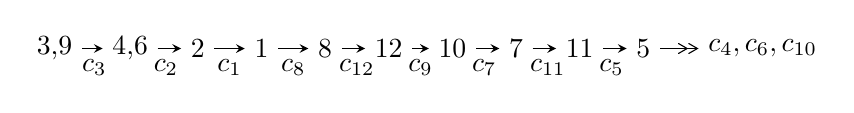
\begin{tikzpicture}[x=23pt, y=7pt]
	% node
	\node (A0) at (-1/8, 0) {3,9};
	\node (A1) at (17/16, 0) {4,6};
	\node (A2) at (17/8, 0) {2};
	\node (A3) at (25/8, 0) {1};
	\node (A4) at (33/8, 0) {8};
	\node (A5) at (41/8, 0) {12};
	\node (A6) at (49/8, 0) {10};
	\node (A7) at (57/8, 0) {7};
	\node (A8) at (65/8, 0) {11};
	\node (A9) at (73/8, 0) {5};
	\node (C1) at (1/2, -1) {$c_{3}$};
	\node (C2) at (13/8, -1) {$c_{2}$};
	\node (C3) at (21/8, -1) {$c_{1}$};
	\node (C4) at (29/8, -1) {$c_{8}$};
	\node (C5) at (37/8, -1) {$c_{12}$};
	\node (C6) at (45/8, -1) {$c_{9}$};
	\node (C7) at (53/8, -1) {$c_{7}$};
	\node (C8) at (61/8, -1) {$c_{11}$};
	\node (C9) at (69/8, -1) {$c_{5}$};
	\node (A10) at (11, 0) {$c_{4},c_{6},c_{10}$};

	% edge
	\draw[->,>=stealth]	
	(A0) edge (A1) (A1) edge (A2) (A2) edge (A3) (A3) edge (A4) (A4) edge (A5) (A5) edge (A6) (A6) edge (A7) (A7) edge (A8) (A8) edge (A9) ;
	\draw[->>,>={angle 60}]	
	(A9) edge (A10);
\end{tikzpicture} \\ 

\end{tabular} \\

\footnotetext{
The image of knot diagram is generated by the software ``\textbf{Draw programme}" developed by Andrew Bartholomew(\url{http://www.layer8.co.uk/maths/draw/index.htm\#Running-draw}), where we modified some parts for our purpose(\url{https://github.com/CATsTAILs/LinksPainter}).
}\phantom \\ \newline 
\centering \textbf{Ideals for irreducible components\footnotemark of $X_{\text{par}}$} 
 
\begin{align*}
I^u_{1}&=\langle 
6.76118\times10^{193} u^{63}+5.01371\times10^{193} u^{62}+\cdots+1.25354\times10^{194} b+4.44874\times10^{194},\\
\phantom{I^u_{1}}&\phantom{= \langle  }2.86519\times10^{194} u^{63}+6.21880\times10^{194} u^{62}+\cdots+7.52124\times10^{194} a+9.81839\times10^{195},\;u^{64}+u^{63}+\cdots+19 u+3\rangle \\
I^u_{2}&=\langle 
-112393648468 u^{22}-311362711897 u^{21}+\cdots+13835100361679 b-17479985966667,\\
\phantom{I^u_{2}}&\phantom{= \langle  }279872528016337 u^{22}+237504248059593 u^{21}+\cdots+525733813743802 a+2170261969973827,\\
\phantom{I^u_{2}}&\phantom{= \langle  }u^{23}- u^{21}+\cdots+6 u+1\rangle \\
\\
\end{align*}
\raggedright * 2 irreducible components of $\dim_{\mathbb{C}}=0$, with total 87 representations.\\
\footnotetext{All coefficients of polynomials are rational numbers. But the coefficients are sometimes approximated in decimal forms when there is not enough margin.}
\newpage
\renewcommand{\arraystretch}{1}
\centering \section*{I. $I^u_{1}= \langle 6.76\times10^{193} u^{63}+5.01\times10^{193} u^{62}+\cdots+1.25\times10^{194} b+4.45\times10^{194},\;2.87\times10^{194} u^{63}+6.22\times10^{194} u^{62}+\cdots+7.52\times10^{194} a+9.82\times10^{195},\;u^{64}+u^{63}+\cdots+19 u+3 \rangle$}
\flushleft \textbf{(i) Arc colorings}\\
\begin{tabular}{m{7pt} m{180pt} m{7pt} m{180pt} }
\flushright $a_{3}=$&$\begin{pmatrix}1\\0\end{pmatrix}$ \\
\flushright $a_{9}=$&$\begin{pmatrix}0\\u\end{pmatrix}$ \\
\flushright $a_{4}=$&$\begin{pmatrix}1\\- u^2\end{pmatrix}$ \\
\flushright $a_{6}=$&$\begin{pmatrix}-0.380947 u^{63}-0.826832 u^{62}+\cdots-59.2801 u-13.0542\\-0.539367 u^{63}-0.399965 u^{62}+\cdots-23.3756 u-3.54894\end{pmatrix}$ \\
\flushright $a_{2}=$&$\begin{pmatrix}0.864918 u^{63}+0.925284 u^{62}+\cdots+43.0012 u+5.72243\\0.869510 u^{63}+0.384944 u^{62}+\cdots+17.0021 u-1.04303\end{pmatrix}$ \\
\flushright $a_{1}=$&$\begin{pmatrix}1.73443 u^{63}+1.31023 u^{62}+\cdots+60.0033 u+4.67940\\0.869510 u^{63}+0.384944 u^{62}+\cdots+17.0021 u-1.04303\end{pmatrix}$ \\
\flushright $a_{8}=$&$\begin{pmatrix}-0.367182 u^{63}-0.631069 u^{62}+\cdots-51.2318 u-11.2742\\0.329774 u^{63}+0.0548480 u^{62}+\cdots-2.95329 u-2.44334\end{pmatrix}$ \\
\flushright $a_{12}=$&$\begin{pmatrix}0.920036 u^{63}+0.918957 u^{62}+\cdots+40.1447 u+4.44983\\0.991980 u^{63}+0.500896 u^{62}+\cdots+22.5982 u+0.226335\end{pmatrix}$ \\
\flushright $a_{10}=$&$\begin{pmatrix}-0.336655 u^{63}-0.477158 u^{62}+\cdots-36.0738 u-7.32788\\-0.606568 u^{63}-0.404583 u^{62}+\cdots-19.9997 u-2.71614\end{pmatrix}$ \\
\flushright $a_{7}=$&$\begin{pmatrix}-0.390211 u^{63}-0.905866 u^{62}+\cdots-53.3726 u-12.0097\\-0.969683 u^{63}-0.116368 u^{62}+\cdots-0.389177 u+6.40660\end{pmatrix}$ \\
\flushright $a_{11}=$&$\begin{pmatrix}0.741182 u^{63}+0.321617 u^{62}+\cdots+10.1253 u-2.13735\\0.0835106 u^{63}+0.0670452 u^{62}+\cdots+1.78701 u-0.325318\end{pmatrix}$ \\
\flushright $a_{5}=$&$\begin{pmatrix}-1.24155 u^{63}-1.19696 u^{62}+\cdots-65.0895 u-11.0387\\-0.376759 u^{63}-0.314282 u^{62}+\cdots-18.4692 u-2.96853\end{pmatrix}$\\&\end{tabular}
\flushleft \textbf{(ii) Obstruction class $= -1$}\\~\\
\flushleft \textbf{(iii) Cusp Shapes $= -6.43385 u^{63}-6.54582 u^{62}+\cdots-289.191 u-67.1645$}\\~\\
\newpage\renewcommand{\arraystretch}{1}
\flushleft \textbf{(iv) u-Polynomials at the component}\newline \\
\begin{tabular}{m{50pt}|m{274pt}}
Crossings & \hspace{64pt}u-Polynomials at each crossing \\
\hline $$\begin{aligned}c_{1}\end{aligned}$$&$\begin{aligned}
&u^{64}+32 u^{63}+\cdots+18 u+1
\end{aligned}$\\
\hline $$\begin{aligned}c_{2},c_{6}\end{aligned}$$&$\begin{aligned}
&u^{64}+16 u^{62}+\cdots-2 u+1
\end{aligned}$\\
\hline $$\begin{aligned}c_{3}\end{aligned}$$&$\begin{aligned}
&u^{64}+u^{63}+\cdots+19 u+3
\end{aligned}$\\
\hline $$\begin{aligned}c_{4}\end{aligned}$$&$\begin{aligned}
&u^{64}+3 u^{63}+\cdots-4170722 u+640748
\end{aligned}$\\
\hline $$\begin{aligned}c_{5},c_{11}\end{aligned}$$&$\begin{aligned}
&u^{64}-43 u^{62}+\cdots-783 u+59
\end{aligned}$\\
\hline $$\begin{aligned}c_{7}\end{aligned}$$&$\begin{aligned}
&u^{64}- u^{63}+\cdots+119493 u+223897
\end{aligned}$\\
\hline $$\begin{aligned}c_{8}\end{aligned}$$&$\begin{aligned}
&u^{64}-5 u^{63}+\cdots+813 u+95
\end{aligned}$\\
\hline $$\begin{aligned}c_{9}\end{aligned}$$&$\begin{aligned}
&u^{64}-13 u^{63}+\cdots-62574 u+5609
\end{aligned}$\\
\hline $$\begin{aligned}c_{10}\end{aligned}$$&$\begin{aligned}
&u^{64}+14 u^{63}+\cdots-360448 u+39592
\end{aligned}$\\
\hline $$\begin{aligned}c_{12}\end{aligned}$$&$\begin{aligned}
&u^{64}+3 u^{63}+\cdots+138 u+49
\end{aligned}$\\
\hline
\end{tabular}\\~\\
\newpage\renewcommand{\arraystretch}{1}
\flushleft \textbf{(v) Riley Polynomials at the component}\newline \\
\begin{tabular}{m{50pt}|m{274pt}}
Crossings & \hspace{64pt}Riley Polynomials at each crossing \\
\hline $$\begin{aligned}c_{1}\end{aligned}$$&$\begin{aligned}
&y^{64}-8 y^{63}+\cdots+18 y+1
\end{aligned}$\\
\hline $$\begin{aligned}c_{2},c_{6}\end{aligned}$$&$\begin{aligned}
&y^{64}+32 y^{63}+\cdots+18 y+1
\end{aligned}$\\
\hline $$\begin{aligned}c_{3}\end{aligned}$$&$\begin{aligned}
&y^{64}+y^{63}+\cdots+167 y+9
\end{aligned}$\\
\hline $$\begin{aligned}c_{4}\end{aligned}$$&$\begin{aligned}
&y^{64}-39 y^{63}+\cdots-7589236264780 y+410557999504
\end{aligned}$\\
\hline $$\begin{aligned}c_{5},c_{11}\end{aligned}$$&$\begin{aligned}
&y^{64}-86 y^{63}+\cdots-103211 y+3481
\end{aligned}$\\
\hline $$\begin{aligned}c_{7}\end{aligned}$$&$\begin{aligned}
&y^{64}-99 y^{63}+\cdots-1572065687631 y+50129866609
\end{aligned}$\\
\hline $$\begin{aligned}c_{8}\end{aligned}$$&$\begin{aligned}
&y^{64}- y^{63}+\cdots+166101 y+9025
\end{aligned}$\\
\hline $$\begin{aligned}c_{9}\end{aligned}$$&$\begin{aligned}
&y^{64}-39 y^{63}+\cdots-766399734 y+31460881
\end{aligned}$\\
\hline $$\begin{aligned}c_{10}\end{aligned}$$&$\begin{aligned}
&y^{64}-116 y^{63}+\cdots+12169918304 y+1567526464
\end{aligned}$\\
\hline $$\begin{aligned}c_{12}\end{aligned}$$&$\begin{aligned}
&y^{64}+9 y^{63}+\cdots+87090 y+2401
\end{aligned}$\\
\hline
\end{tabular}\\~\\
\newpage\flushleft \textbf{(vi) Complex Volumes and Cusp Shapes}
$$\begin{array}{c|c|c}  
\text{Solutions to }I^u_{1}& \I (\text{vol} + \sqrt{-1}CS) & \text{Cusp shape}\\
 \hline 
\begin{aligned}
u &= \phantom{-}0.768439 + 0.710097 I \\
a &= \phantom{-}1.306620 + 0.123877 I \\
b &= -0.72129 - 1.34035 I\end{aligned}
 & -10.46510 + 7.62597 I & \phantom{-0.000000 } 0 \\ \hline\begin{aligned}
u &= \phantom{-}0.768439 - 0.710097 I \\
a &= \phantom{-}1.306620 - 0.123877 I \\
b &= -0.72129 + 1.34035 I\end{aligned}
 & -10.46510 - 7.62597 I & \phantom{-0.000000 } 0 \\ \hline\begin{aligned}
u &= -0.085218 + 1.067950 I \\
a &= -0.423774 - 0.836346 I \\
b &= -0.255634 - 0.976959 I\end{aligned}
 & -4.35206 + 0.82760 I & \phantom{-0.000000 } 0 \\ \hline\begin{aligned}
u &= -0.085218 - 1.067950 I \\
a &= -0.423774 + 0.836346 I \\
b &= -0.255634 + 0.976959 I\end{aligned}
 & -4.35206 - 0.82760 I & \phantom{-0.000000 } 0 \\ \hline\begin{aligned}
u &= \phantom{-}0.266521 + 0.888631 I \\
a &= \phantom{-}0.693375 - 0.164357 I \\
b &= -0.451141 + 1.243390 I\end{aligned}
 & -3.60138 + 1.26061 I & -9.53908 - 0.36965 I \\ \hline\begin{aligned}
u &= \phantom{-}0.266521 - 0.888631 I \\
a &= \phantom{-}0.693375 + 0.164357 I \\
b &= -0.451141 - 1.243390 I\end{aligned}
 & -3.60138 - 1.26061 I & -9.53908 + 0.36965 I \\ \hline\begin{aligned}
u &= \phantom{-}0.455110 + 0.994145 I \\
a &= \phantom{-}0.733351 + 0.024556 I \\
b &= \phantom{-}0.492807 - 1.144750 I\end{aligned}
 & -11.57250 - 2.78285 I & \phantom{-0.000000 } 0 \\ \hline\begin{aligned}
u &= \phantom{-}0.455110 - 0.994145 I \\
a &= \phantom{-}0.733351 - 0.024556 I \\
b &= \phantom{-}0.492807 + 1.144750 I\end{aligned}
 & -11.57250 + 2.78285 I & \phantom{-0.000000 } 0 \\ \hline\begin{aligned}
u &= \phantom{-}0.835939 + 0.288434 I \\
a &= -0.858019 - 0.218506 I \\
b &= \phantom{-}0.546312 + 0.216534 I\end{aligned}
 & \phantom{-}1.46270 + 0.81103 I & \phantom{-}3.71659 + 0.11699 I \\ \hline\begin{aligned}
u &= \phantom{-}0.835939 - 0.288434 I \\
a &= -0.858019 + 0.218506 I \\
b &= \phantom{-}0.546312 - 0.216534 I\end{aligned}
 & \phantom{-}1.46270 - 0.81103 I & \phantom{-}3.71659 - 0.11699 I\\
 \hline 
 \end{array}$$\newpage$$\begin{array}{c|c|c}  
\text{Solutions to }I^u_{1}& \I (\text{vol} + \sqrt{-1}CS) & \text{Cusp shape}\\
 \hline 
\begin{aligned}
u &= -0.971832 + 0.575905 I \\
a &= \phantom{-}0.795059 - 0.858262 I \\
b &= -0.071970 + 0.666140 I\end{aligned}
 & -0.71782 - 4.52201 I & \phantom{-0.000000 } 0 \\ \hline\begin{aligned}
u &= -0.971832 - 0.575905 I \\
a &= \phantom{-}0.795059 + 0.858262 I \\
b &= -0.071970 - 0.666140 I\end{aligned}
 & -0.71782 + 4.52201 I & \phantom{-0.000000 } 0 \\ \hline\begin{aligned}
u &= \phantom{-}0.618813 + 0.970738 I \\
a &= -0.607323 + 0.738340 I \\
b &= \phantom{-}0.341775 + 1.178830 I\end{aligned}
 & -3.60210 + 6.30080 I & \phantom{-0.000000 } 0 \\ \hline\begin{aligned}
u &= \phantom{-}0.618813 - 0.970738 I \\
a &= -0.607323 - 0.738340 I \\
b &= \phantom{-}0.341775 - 1.178830 I\end{aligned}
 & -3.60210 - 6.30080 I & \phantom{-0.000000 } 0 \\ \hline\begin{aligned}
u &= \phantom{-}0.952500 + 0.649719 I \\
a &= \phantom{-}0.456188 - 0.728196 I \\
b &= -0.672285 + 0.580916 I\end{aligned}
 & \phantom{-}2.58365 + 2.09320 I & \phantom{-0.000000 } 0 \\ \hline\begin{aligned}
u &= \phantom{-}0.952500 - 0.649719 I \\
a &= \phantom{-}0.456188 + 0.728196 I \\
b &= -0.672285 - 0.580916 I\end{aligned}
 & \phantom{-}2.58365 - 2.09320 I & \phantom{-0.000000 } 0 \\ \hline\begin{aligned}
u &= \phantom{-}0.021851 + 0.821787 I \\
a &= \phantom{-}0.47182 - 2.13552 I \\
b &= \phantom{-}0.489476 - 0.207876 I\end{aligned}
 & -8.94146 - 1.47584 I & -7.02830 + 5.13134 I \\ \hline\begin{aligned}
u &= \phantom{-}0.021851 - 0.821787 I \\
a &= \phantom{-}0.47182 + 2.13552 I \\
b &= \phantom{-}0.489476 + 0.207876 I\end{aligned}
 & -8.94146 + 1.47584 I & -7.02830 - 5.13134 I \\ \hline\begin{aligned}
u &= -0.468002 + 1.129190 I \\
a &= -0.136369 - 0.174368 I \\
b &= \phantom{-}0.10048 + 1.51887 I\end{aligned}
 & -16.4681 - 4.7254 I & \phantom{-0.000000 } 0 \\ \hline\begin{aligned}
u &= -0.468002 - 1.129190 I \\
a &= -0.136369 + 0.174368 I \\
b &= \phantom{-}0.10048 - 1.51887 I\end{aligned}
 & -16.4681 + 4.7254 I & \phantom{-0.000000 } 0\\
 \hline 
 \end{array}$$\newpage$$\begin{array}{c|c|c}  
\text{Solutions to }I^u_{1}& \I (\text{vol} + \sqrt{-1}CS) & \text{Cusp shape}\\
 \hline 
\begin{aligned}
u &= -0.830809 + 0.908495 I \\
a &= \phantom{-}1.53629 + 0.69226 I \\
b &= -0.627832 + 1.024980 I\end{aligned}
 & \phantom{-}1.28045 - 7.16483 I & \phantom{-0.000000 } 0 \\ \hline\begin{aligned}
u &= -0.830809 - 0.908495 I \\
a &= \phantom{-}1.53629 - 0.69226 I \\
b &= -0.627832 - 1.024980 I\end{aligned}
 & \phantom{-}1.28045 + 7.16483 I & \phantom{-0.000000 } 0 \\ \hline\begin{aligned}
u &= \phantom{-}0.102197 + 0.756108 I \\
a &= -0.999058 + 0.316929 I \\
b &= \phantom{-}0.650916 + 0.954374 I\end{aligned}
 & \phantom{-}0.31001 + 2.61678 I & \phantom{-}0.776084 - 0.171136 I \\ \hline\begin{aligned}
u &= \phantom{-}0.102197 - 0.756108 I \\
a &= -0.999058 - 0.316929 I \\
b &= \phantom{-}0.650916 - 0.954374 I\end{aligned}
 & \phantom{-}0.31001 - 2.61678 I & \phantom{-}0.776084 + 0.171136 I \\ \hline\begin{aligned}
u &= -1.006830 + 0.792686 I \\
a &= \phantom{-}0.941730 + 0.113880 I \\
b &= -0.718433 - 0.167055 I\end{aligned}
 & -0.05240 - 5.34782 I & \phantom{-0.000000 } 0 \\ \hline\begin{aligned}
u &= -1.006830 - 0.792686 I \\
a &= \phantom{-}0.941730 - 0.113880 I \\
b &= -0.718433 + 0.167055 I\end{aligned}
 & -0.05240 + 5.34782 I & \phantom{-0.000000 } 0 \\ \hline\begin{aligned}
u &= -0.347978 + 0.595874 I \\
a &= \phantom{-}2.33082 + 0.15889 I \\
b &= -0.573908 + 0.916885 I\end{aligned}
 & -2.27384 - 4.56530 I & -7.78284 + 7.48206 I \\ \hline\begin{aligned}
u &= -0.347978 - 0.595874 I \\
a &= \phantom{-}2.33082 - 0.15889 I \\
b &= -0.573908 - 0.916885 I\end{aligned}
 & -2.27384 + 4.56530 I & -7.78284 - 7.48206 I \\ \hline\begin{aligned}
u &= \phantom{-}0.983563 + 0.949818 I \\
a &= \phantom{-}1.52104 - 0.72824 I \\
b &= -0.623974 - 0.099517 I\end{aligned}
 & -9.24473 - 1.84302 I & \phantom{-0.000000 } 0 \\ \hline\begin{aligned}
u &= \phantom{-}0.983563 - 0.949818 I \\
a &= \phantom{-}1.52104 + 0.72824 I \\
b &= -0.623974 + 0.099517 I\end{aligned}
 & -9.24473 + 1.84302 I & \phantom{-0.000000 } 0\\
 \hline 
 \end{array}$$\newpage$$\begin{array}{c|c|c}  
\text{Solutions to }I^u_{1}& \I (\text{vol} + \sqrt{-1}CS) & \text{Cusp shape}\\
 \hline 
\begin{aligned}
u &= \phantom{-}0.498586 + 0.342899 I \\
a &= -3.69984 - 2.03368 I \\
b &= \phantom{-}0.449391 + 1.143210 I\end{aligned}
 & -11.89270 + 5.18300 I & -9.77291 - 9.94345 I \\ \hline\begin{aligned}
u &= \phantom{-}0.498586 - 0.342899 I \\
a &= -3.69984 + 2.03368 I \\
b &= \phantom{-}0.449391 - 1.143210 I\end{aligned}
 & -11.89270 - 5.18300 I & -9.77291 + 9.94345 I \\ \hline\begin{aligned}
u &= -0.461857 + 0.379511 I \\
a &= -1.44331 - 0.07225 I \\
b &= \phantom{-}0.486831 - 1.275810 I\end{aligned}
 & -1.85538 - 2.97884 I & -6.59140 + 7.67980 I \\ \hline\begin{aligned}
u &= -0.461857 - 0.379511 I \\
a &= -1.44331 + 0.07225 I \\
b &= \phantom{-}0.486831 + 1.275810 I\end{aligned}
 & -1.85538 + 2.97884 I & -6.59140 - 7.67980 I \\ \hline\begin{aligned}
u &= -1.12543 + 0.86119 I \\
a &= -1.003630 - 0.572524 I \\
b &= \phantom{-}0.721686 + 0.659860 I\end{aligned}
 & \phantom{-}0.148717 - 0.150459 I & \phantom{-0.000000 } 0 \\ \hline\begin{aligned}
u &= -1.12543 - 0.86119 I \\
a &= -1.003630 + 0.572524 I \\
b &= \phantom{-}0.721686 - 0.659860 I\end{aligned}
 & \phantom{-}0.148717 + 0.150459 I & \phantom{-0.000000 } 0 \\ \hline\begin{aligned}
u &= \phantom{-}0.98638 + 1.04285 I \\
a &= -1.092850 + 0.417343 I \\
b &= \phantom{-}1.118790 - 0.379740 I\end{aligned}
 & -9.44514 + 9.24996 I & \phantom{-0.000000 } 0 \\ \hline\begin{aligned}
u &= \phantom{-}0.98638 - 1.04285 I \\
a &= -1.092850 - 0.417343 I \\
b &= \phantom{-}1.118790 + 0.379740 I\end{aligned}
 & -9.44514 - 9.24996 I & \phantom{-0.000000 } 0 \\ \hline\begin{aligned}
u &= \phantom{-}1.44274 + 0.02938 I \\
a &= -0.615836 + 0.495319 I \\
b &= \phantom{-}0.071795 - 0.805712 I\end{aligned}
 & -0.144341 + 1.401570 I & \phantom{-0.000000 } 0 \\ \hline\begin{aligned}
u &= \phantom{-}1.44274 - 0.02938 I \\
a &= -0.615836 - 0.495319 I \\
b &= \phantom{-}0.071795 + 0.805712 I\end{aligned}
 & -0.144341 - 1.401570 I & \phantom{-0.000000 } 0\\
 \hline 
 \end{array}$$\newpage$$\begin{array}{c|c|c}  
\text{Solutions to }I^u_{1}& \I (\text{vol} + \sqrt{-1}CS) & \text{Cusp shape}\\
 \hline 
\begin{aligned}
u &= -0.518307 + 0.185402 I \\
a &= -0.354206 + 0.642889 I \\
b &= \phantom{-}0.865746 - 0.532757 I\end{aligned}
 & \phantom{-}1.10608 - 3.36124 I & -0.42621 + 9.54804 I \\ \hline\begin{aligned}
u &= -0.518307 - 0.185402 I \\
a &= -0.354206 - 0.642889 I \\
b &= \phantom{-}0.865746 + 0.532757 I\end{aligned}
 & \phantom{-}1.10608 + 3.36124 I & -0.42621 - 9.54804 I \\ \hline\begin{aligned}
u &= \phantom{-}0.344648 + 0.412119 I \\
a &= \phantom{-}3.43307 - 3.90269 I \\
b &= \phantom{-}0.125752 + 0.298631 I\end{aligned}
 & -9.08308 - 1.54040 I & -3.52047 + 8.43213 I \\ \hline\begin{aligned}
u &= \phantom{-}0.344648 - 0.412119 I \\
a &= \phantom{-}3.43307 + 3.90269 I \\
b &= \phantom{-}0.125752 - 0.298631 I\end{aligned}
 & -9.08308 + 1.54040 I & -3.52047 - 8.43213 I \\ \hline\begin{aligned}
u &= -1.14020 + 0.92833 I \\
a &= -0.991241 - 0.285891 I \\
b &= \phantom{-}0.309850 - 1.050050 I\end{aligned}
 & -1.66777 - 3.20908 I & \phantom{-0.000000 } 0 \\ \hline\begin{aligned}
u &= -1.14020 - 0.92833 I \\
a &= -0.991241 + 0.285891 I \\
b &= \phantom{-}0.309850 + 1.050050 I\end{aligned}
 & -1.66777 + 3.20908 I & \phantom{-0.000000 } 0 \\ \hline\begin{aligned}
u &= -0.227253 + 0.454347 I \\
a &= -0.150236 - 1.032800 I \\
b &= -0.350045 + 0.327230 I\end{aligned}
 & -1.26856 + 0.70605 I & -5.19223 - 1.71159 I \\ \hline\begin{aligned}
u &= -0.227253 - 0.454347 I \\
a &= -0.150236 + 1.032800 I \\
b &= -0.350045 - 0.327230 I\end{aligned}
 & -1.26856 - 0.70605 I & -5.19223 + 1.71159 I \\ \hline\begin{aligned}
u &= -0.276652 + 0.303262 I \\
a &= \phantom{-}1.48929 + 0.35722 I \\
b &= -1.58452 - 0.40190 I\end{aligned}
 & -7.09270 - 0.18320 I & -8.5918 + 26.1881 I \\ \hline\begin{aligned}
u &= -0.276652 - 0.303262 I \\
a &= \phantom{-}1.48929 - 0.35722 I \\
b &= -1.58452 + 0.40190 I\end{aligned}
 & -7.09270 + 0.18320 I & -8.5918 - 26.1881 I\\
 \hline 
 \end{array}$$\newpage$$\begin{array}{c|c|c}  
\text{Solutions to }I^u_{1}& \I (\text{vol} + \sqrt{-1}CS) & \text{Cusp shape}\\
 \hline 
\begin{aligned}
u &= \phantom{-}1.25213 + 1.08328 I \\
a &= -1.59960 + 0.05491 I \\
b &= \phantom{-}0.672809 + 1.012270 I\end{aligned}
 & -0.91338 + 5.51890 I & \phantom{-0.000000 } 0 \\ \hline\begin{aligned}
u &= \phantom{-}1.25213 - 1.08328 I \\
a &= -1.59960 - 0.05491 I \\
b &= \phantom{-}0.672809 - 1.012270 I\end{aligned}
 & -0.91338 - 5.51890 I & \phantom{-0.000000 } 0 \\ \hline\begin{aligned}
u &= -0.156228 + 0.290874 I \\
a &= \phantom{-}0.21881 - 3.26254 I \\
b &= -0.213772 - 0.956901 I\end{aligned}
 & -1.62143 - 1.10348 I & -5.00798 + 3.54749 I \\ \hline\begin{aligned}
u &= -0.156228 - 0.290874 I \\
a &= \phantom{-}0.21881 + 3.26254 I \\
b &= -0.213772 + 0.956901 I\end{aligned}
 & -1.62143 + 1.10348 I & -5.00798 - 3.54749 I \\ \hline\begin{aligned}
u &= -1.16098 + 1.20032 I \\
a &= -1.412120 - 0.001483 I \\
b &= \phantom{-}0.69640 - 1.25090 I\end{aligned}
 & -12.1872 - 15.7252 I & \phantom{-0.000000 } 0 \\ \hline\begin{aligned}
u &= -1.16098 - 1.20032 I \\
a &= -1.412120 + 0.001483 I \\
b &= \phantom{-}0.69640 + 1.25090 I\end{aligned}
 & -12.1872 + 15.7252 I & \phantom{-0.000000 } 0 \\ \hline\begin{aligned}
u &= \phantom{-}1.21102 + 1.16930 I \\
a &= \phantom{-}1.160920 - 0.049651 I \\
b &= -0.512568 - 1.188460 I\end{aligned}
 & -3.03377 + 10.06590 I & \phantom{-0.000000 } 0 \\ \hline\begin{aligned}
u &= \phantom{-}1.21102 - 1.16930 I \\
a &= \phantom{-}1.160920 + 0.049651 I \\
b &= -0.512568 + 1.188460 I\end{aligned}
 & -3.03377 - 10.06590 I & \phantom{-0.000000 } 0 \\ \hline\begin{aligned}
u &= \phantom{-}0.61897 + 1.71494 I \\
a &= -0.305411 - 0.225319 I \\
b &= \phantom{-}0.180451 - 1.014300 I\end{aligned}
 & -4.44894 - 0.47351 I & \phantom{-0.000000 } 0 \\ \hline\begin{aligned}
u &= \phantom{-}0.61897 - 1.71494 I \\
a &= -0.305411 + 0.225319 I \\
b &= \phantom{-}0.180451 + 1.014300 I\end{aligned}
 & -4.44894 + 0.47351 I & \phantom{-0.000000 } 0\\
 \hline 
 \end{array}$$\newpage$$\begin{array}{c|c|c}  
\text{Solutions to }I^u_{1}& \I (\text{vol} + \sqrt{-1}CS) & \text{Cusp shape}\\
 \hline 
\begin{aligned}
u &= -1.74962 + 0.59173 I \\
a &= \phantom{-}1.25972 - 0.65598 I \\
b &= -0.450065 + 1.179190 I\end{aligned}
 & -12.53600 - 2.18533 I & \phantom{-0.000000 } 0 \\ \hline\begin{aligned}
u &= -1.74962 - 0.59173 I \\
a &= \phantom{-}1.25972 + 0.65598 I \\
b &= -0.450065 - 1.179190 I\end{aligned}
 & -12.53600 + 2.18533 I & \phantom{-0.000000 } 0 \\ \hline\begin{aligned}
u &= -1.33222 + 1.51909 I \\
a &= \phantom{-}0.511399 + 0.352829 I \\
b &= -0.493832 - 1.176170 I\end{aligned}
 & -12.21100 + 6.27838 I & \phantom{-0.000000 } 0 \\ \hline\begin{aligned}
u &= -1.33222 - 1.51909 I \\
a &= \phantom{-}0.511399 - 0.352829 I \\
b &= -0.493832 + 1.176170 I\end{aligned}
 & -12.21100 - 6.27838 I & \phantom{-0.000000 } 0\\
 \hline 
 \end{array}$$\newpage\newpage\renewcommand{\arraystretch}{1}
\centering \section*{II. $I^u_{2}= \langle -1.12\times10^{11} u^{22}-3.11\times10^{11} u^{21}+\cdots+1.38\times10^{13} b-1.75\times10^{13},\;2.80\times10^{14} u^{22}+2.38\times10^{14} u^{21}+\cdots+5.26\times10^{14} a+2.17\times10^{15},\;u^{23}- u^{21}+\cdots+6 u+1 \rangle$}
\flushleft \textbf{(i) Arc colorings}\\
\begin{tabular}{m{7pt} m{180pt} m{7pt} m{180pt} }
\flushright $a_{3}=$&$\begin{pmatrix}1\\0\end{pmatrix}$ \\
\flushright $a_{9}=$&$\begin{pmatrix}0\\u\end{pmatrix}$ \\
\flushright $a_{4}=$&$\begin{pmatrix}1\\- u^2\end{pmatrix}$ \\
\flushright $a_{6}=$&$\begin{pmatrix}-0.532346 u^{22}-0.451758 u^{21}+\cdots-3.94607 u-4.12806\\0.00812380 u^{22}+0.0225053 u^{21}+\cdots-1.76899 u+1.26345\end{pmatrix}$ \\
\flushright $a_{2}=$&$\begin{pmatrix}-0.576639 u^{22}-0.0415103 u^{21}+\cdots+0.865302 u-4.15266\\0.523266 u^{22}-0.0991113 u^{21}+\cdots+0.406061 u+2.45807\end{pmatrix}$ \\
\flushright $a_{1}=$&$\begin{pmatrix}-0.0533735 u^{22}-0.140622 u^{21}+\cdots+1.27136 u-1.69459\\0.523266 u^{22}-0.0991113 u^{21}+\cdots+0.406061 u+2.45807\end{pmatrix}$ \\
\flushright $a_{8}=$&$\begin{pmatrix}-0.240226 u^{22}-0.000150414 u^{21}+\cdots-2.50811 u+0.149221\\-0.126360 u^{22}+0.105650 u^{21}+\cdots-0.0810748 u-0.916657\end{pmatrix}$ \\
\flushright $a_{12}=$&$\begin{pmatrix}-0.578843 u^{22}-0.170099 u^{21}+\cdots-0.0318002 u-4.29328\\0.229238 u^{22}-0.0424956 u^{21}+\cdots-0.296275 u+2.42859\end{pmatrix}$ \\
\flushright $a_{10}=$&$\begin{pmatrix}-0.201365 u^{22}+0.284014 u^{21}+\cdots-1.93952 u+2.76031\\-0.0989915 u^{22}+0.379233 u^{21}+\cdots+2.77408 u-1.41057\end{pmatrix}$ \\
\flushright $a_{7}=$&$\begin{pmatrix}-1.57884 u^{22}-0.170099 u^{21}+\cdots-1.03180 u-10.2933\\0.718281 u^{22}-0.215517 u^{21}+\cdots-2.43939 u+4.91339\end{pmatrix}$ \\
\flushright $a_{11}=$&$\begin{pmatrix}0.631324 u^{22}+0.428112 u^{21}+\cdots+4.76746 u+2.95129\\-0.107101 u^{22}+0.00114053 u^{21}+\cdots+1.94761 u-0.0866821\end{pmatrix}$ \\
\flushright $a_{5}=$&$\begin{pmatrix}0.284014 u^{22}+0.0456181 u^{21}+\cdots+3.96851 u+1.20137\\0.206212 u^{22}+0.164773 u^{21}+\cdots-1.26608 u+0.609948\end{pmatrix}$\\&\end{tabular}
\flushleft \textbf{(ii) Obstruction class $= 1$}\\~\\
\flushleft \textbf{(iii) Cusp Shapes $= -\frac{355563029923215}{262866906871901} u^{22}-\frac{201540020728255}{262866906871901} u^{21}+\cdots+\frac{1754556307346636}{262866906871901} u-\frac{6210727541948044}{262866906871901}$}\\~\\
\newpage\renewcommand{\arraystretch}{1}
\flushleft \textbf{(iv) u-Polynomials at the component}\newline \\
\begin{tabular}{m{50pt}|m{274pt}}
Crossings & \hspace{64pt}u-Polynomials at each crossing \\
\hline $$\begin{aligned}c_{1}\end{aligned}$$&$\begin{aligned}
&u^{23}-9 u^{22}+\cdots-11 u+1
\end{aligned}$\\
\hline $$\begin{aligned}c_{2}\end{aligned}$$&$\begin{aligned}
&u^{23}- u^{22}+\cdots+u-1
\end{aligned}$\\
\hline $$\begin{aligned}c_{3}\end{aligned}$$&$\begin{aligned}
&u^{23}- u^{21}+\cdots+6 u+1
\end{aligned}$\\
\hline $$\begin{aligned}c_{4}\end{aligned}$$&$\begin{aligned}
&u^{23}-3 u^{21}+\cdots+6 u+4
\end{aligned}$\\
\hline $$\begin{aligned}c_{5}\end{aligned}$$&$\begin{aligned}
&u^{23}+u^{22}+\cdots+4 u+1
\end{aligned}$\\
\hline $$\begin{aligned}c_{6}\end{aligned}$$&$\begin{aligned}
&u^{23}+u^{22}+\cdots+u+1
\end{aligned}$\\
\hline $$\begin{aligned}c_{7}\end{aligned}$$&$\begin{aligned}
&u^{23}+2 u^{22}+\cdots-6 u+1
\end{aligned}$\\
\hline $$\begin{aligned}c_{8}\end{aligned}$$&$\begin{aligned}
&u^{23}-4 u^{21}+\cdots+6 u+1
\end{aligned}$\\
\hline $$\begin{aligned}c_{9}\end{aligned}$$&$\begin{aligned}
&u^{23}-6 u^{22}+\cdots+3 u+1
\end{aligned}$\\
\hline $$\begin{aligned}c_{10}\end{aligned}$$&$\begin{aligned}
&u^{23}+15 u^{22}+\cdots+4 u+8
\end{aligned}$\\
\hline $$\begin{aligned}c_{11}\end{aligned}$$&$\begin{aligned}
&u^{23}- u^{22}+\cdots+4 u-1
\end{aligned}$\\
\hline $$\begin{aligned}c_{12}\end{aligned}$$&$\begin{aligned}
&u^{23}+2 u^{22}+\cdots-3 u+1
\end{aligned}$\\
\hline
\end{tabular}\\~\\
\newpage\renewcommand{\arraystretch}{1}
\flushleft \textbf{(v) Riley Polynomials at the component}\newline \\
\begin{tabular}{m{50pt}|m{274pt}}
Crossings & \hspace{64pt}Riley Polynomials at each crossing \\
\hline $$\begin{aligned}c_{1}\end{aligned}$$&$\begin{aligned}
&y^{23}+y^{22}+\cdots-15 y-1
\end{aligned}$\\
\hline $$\begin{aligned}c_{2},c_{6}\end{aligned}$$&$\begin{aligned}
&y^{23}+9 y^{22}+\cdots-11 y-1
\end{aligned}$\\
\hline $$\begin{aligned}c_{3}\end{aligned}$$&$\begin{aligned}
&y^{23}-2 y^{22}+\cdots+36 y-1
\end{aligned}$\\
\hline $$\begin{aligned}c_{4}\end{aligned}$$&$\begin{aligned}
&y^{23}-6 y^{22}+\cdots-308 y-16
\end{aligned}$\\
\hline $$\begin{aligned}c_{5},c_{11}\end{aligned}$$&$\begin{aligned}
&y^{23}-25 y^{22}+\cdots+14 y-1
\end{aligned}$\\
\hline $$\begin{aligned}c_{7}\end{aligned}$$&$\begin{aligned}
&y^{23}-18 y^{22}+\cdots-14 y-1
\end{aligned}$\\
\hline $$\begin{aligned}c_{8}\end{aligned}$$&$\begin{aligned}
&y^{23}-8 y^{22}+\cdots+22 y-1
\end{aligned}$\\
\hline $$\begin{aligned}c_{9}\end{aligned}$$&$\begin{aligned}
&y^{23}-18 y^{22}+\cdots+17 y-1
\end{aligned}$\\
\hline $$\begin{aligned}c_{10}\end{aligned}$$&$\begin{aligned}
&y^{23}-23 y^{22}+\cdots-112 y-64
\end{aligned}$\\
\hline $$\begin{aligned}c_{12}\end{aligned}$$&$\begin{aligned}
&y^{23}-2 y^{22}+\cdots-7 y-1
\end{aligned}$\\
\hline
\end{tabular}\\~\\
\newpage\flushleft \textbf{(vi) Complex Volumes and Cusp Shapes}
$$\begin{array}{c|c|c}  
\text{Solutions to }I^u_{2}& \I (\text{vol} + \sqrt{-1}CS) & \text{Cusp shape}\\
 \hline 
\begin{aligned}
u &= -0.893750 + 0.421240 I \\
a &= -0.700987 + 0.971805 I \\
b &= \phantom{-}0.424483 - 0.573628 I\end{aligned}
 & -0.19060 - 5.12115 I & \phantom{-}0.52825 + 10.04685 I \\ \hline\begin{aligned}
u &= -0.893750 - 0.421240 I \\
a &= -0.700987 - 0.971805 I \\
b &= \phantom{-}0.424483 + 0.573628 I\end{aligned}
 & -0.19060 + 5.12115 I & \phantom{-}0.52825 - 10.04685 I \\ \hline\begin{aligned}
u &= \phantom{-}1.009380 + 0.144862 I \\
a &= \phantom{-}0.501893 - 0.040694 I \\
b &= -0.582203 + 0.603687 I\end{aligned}
 & \phantom{-}1.18763 - 2.35933 I & -0.54441 + 2.81335 I \\ \hline\begin{aligned}
u &= \phantom{-}1.009380 - 0.144862 I \\
a &= \phantom{-}0.501893 + 0.040694 I \\
b &= -0.582203 - 0.603687 I\end{aligned}
 & \phantom{-}1.18763 + 2.35933 I & -0.54441 - 2.81335 I \\ \hline\begin{aligned}
u &= \phantom{-}0.824076 + 0.431980 I \\
a &= -0.31656 + 1.78055 I \\
b &= \phantom{-}0.434403 - 1.159370 I\end{aligned}
 & -11.75970 - 4.28995 I & -7.55896 + 1.61429 I \\ \hline\begin{aligned}
u &= \phantom{-}0.824076 - 0.431980 I \\
a &= -0.31656 - 1.78055 I \\
b &= \phantom{-}0.434403 + 1.159370 I\end{aligned}
 & -11.75970 + 4.28995 I & -7.55896 - 1.61429 I \\ \hline\begin{aligned}
u &= -0.432840 + 0.804291 I \\
a &= \phantom{-}1.264390 - 0.010317 I \\
b &= -0.733090 + 0.984673 I\end{aligned}
 & -0.29640 - 3.14054 I & -6.31334 + 6.17687 I \\ \hline\begin{aligned}
u &= -0.432840 - 0.804291 I \\
a &= \phantom{-}1.264390 + 0.010317 I \\
b &= -0.733090 - 0.984673 I\end{aligned}
 & -0.29640 + 3.14054 I & -6.31334 - 6.17687 I \\ \hline\begin{aligned}
u &= -0.448748 + 0.721348 I \\
a &= -1.93684 - 3.19433 I \\
b &= \phantom{-}0.237145 - 0.577461 I\end{aligned}
 & -9.30020 + 1.18087 I & -13.7807 + 7.4362 I \\ \hline\begin{aligned}
u &= -0.448748 - 0.721348 I \\
a &= -1.93684 + 3.19433 I \\
b &= \phantom{-}0.237145 + 0.577461 I\end{aligned}
 & -9.30020 - 1.18087 I & -13.7807 - 7.4362 I\\
 \hline 
 \end{array}$$\newpage$$\begin{array}{c|c|c}  
\text{Solutions to }I^u_{2}& \I (\text{vol} + \sqrt{-1}CS) & \text{Cusp shape}\\
 \hline 
\begin{aligned}
u &= \phantom{-}0.137895 + 0.681215 I \\
a &= -0.647316 - 0.323996 I \\
b &= \phantom{-}0.098638 - 1.232580 I\end{aligned}
 & -2.98206 + 2.14068 I & -7.34511 - 5.88395 I \\ \hline\begin{aligned}
u &= \phantom{-}0.137895 - 0.681215 I \\
a &= -0.647316 + 0.323996 I \\
b &= \phantom{-}0.098638 + 1.232580 I\end{aligned}
 & -2.98206 - 2.14068 I & -7.34511 + 5.88395 I \\ \hline\begin{aligned}
u &= -1.108090 + 0.692297 I \\
a &= \phantom{-}1.77762 + 0.17325 I \\
b &= -0.617221 + 1.022100 I\end{aligned}
 & \phantom{-}0.25873 - 5.53788 I & -1.35642 + 5.56127 I \\ \hline\begin{aligned}
u &= -1.108090 - 0.692297 I \\
a &= \phantom{-}1.77762 - 0.17325 I \\
b &= -0.617221 - 1.022100 I\end{aligned}
 & \phantom{-}0.25873 + 5.53788 I & -1.35642 - 5.56127 I \\ \hline\begin{aligned}
u &= \phantom{-}1.252020 + 0.409058 I \\
a &= \phantom{-}1.013030 - 0.856909 I \\
b &= -0.590775 + 0.675547 I\end{aligned}
 & \phantom{-}1.39201 + 0.69958 I & \phantom{-}0.150882 - 0.471117 I \\ \hline\begin{aligned}
u &= \phantom{-}1.252020 - 0.409058 I \\
a &= \phantom{-}1.013030 + 0.856909 I \\
b &= -0.590775 - 0.675547 I\end{aligned}
 & \phantom{-}1.39201 - 0.69958 I & \phantom{-}0.150882 + 0.471117 I \\ \hline\begin{aligned}
u &= -0.114607 + 1.393680 I \\
a &= \phantom{-}0.013743 - 0.511692 I \\
b &= -0.239456 - 0.903215 I\end{aligned}
 & -3.69072 + 1.05790 I & -1.89355 - 6.61055 I \\ \hline\begin{aligned}
u &= -0.114607 - 1.393680 I \\
a &= \phantom{-}0.013743 + 0.511692 I \\
b &= -0.239456 + 0.903215 I\end{aligned}
 & -3.69072 - 1.05790 I & -1.89355 + 6.61055 I \\ \hline\begin{aligned}
u &= -1.062860 + 0.913991 I \\
a &= -0.401149 - 0.557990 I \\
b &= \phantom{-}0.639569 + 0.734356 I\end{aligned}
 & \phantom{-}0.88359 - 3.30259 I & -3.25538 + 1.96589 I \\ \hline\begin{aligned}
u &= -1.062860 - 0.913991 I \\
a &= -0.401149 + 0.557990 I \\
b &= \phantom{-}0.639569 - 0.734356 I\end{aligned}
 & \phantom{-}0.88359 + 3.30259 I & -3.25538 - 1.96589 I\\
 \hline 
 \end{array}$$\newpage$$\begin{array}{c|c|c}  
\text{Solutions to }I^u_{2}& \I (\text{vol} + \sqrt{-1}CS) & \text{Cusp shape}\\
 \hline 
\begin{aligned}
u &= \phantom{-}0.91918 + 1.12261 I \\
a &= -1.36761 + 0.59069 I \\
b &= \phantom{-}0.640606 + 0.971353 I\end{aligned}
 & \phantom{-}0.12927 + 8.32658 I & -4.10216 - 9.00086 I \\ \hline\begin{aligned}
u &= \phantom{-}0.91918 - 1.12261 I \\
a &= -1.36761 - 0.59069 I \\
b &= \phantom{-}0.640606 - 0.971353 I\end{aligned}
 & \phantom{-}0.12927 - 8.32658 I & -4.10216 + 9.00086 I \\ \hline\begin{aligned}
u &= -0.163309\phantom{ +0.000000I} \\
a &= -3.40044\phantom{ +0.000000I} \\
b &= \phantom{-}1.57580\phantom{ +0.000000I}\end{aligned}
 & -7.19079\phantom{ +0.000000I} & -25.0580\phantom{ +0.000000I}\\
 \hline 
 \end{array}$$\newpage
\newpage\renewcommand{\arraystretch}{1}
\centering \section*{ III. u-Polynomials}
\begin{tabular}{m{50pt}|m{274pt}}
Crossings & \hspace{64pt}u-Polynomials at each crossing \\
\hline $$\begin{aligned}c_{1}\end{aligned}$$&$\begin{aligned}
&(u^{23}-9 u^{22}+\cdots-11 u+1)(u^{64}+32 u^{63}+\cdots+18 u+1)
\end{aligned}$\\
\hline $$\begin{aligned}c_{2}\end{aligned}$$&$\begin{aligned}
&(u^{23}- u^{22}+\cdots+u-1)(u^{64}+16 u^{62}+\cdots-2 u+1)
\end{aligned}$\\
\hline $$\begin{aligned}c_{3}\end{aligned}$$&$\begin{aligned}
&(u^{23}- u^{21}+\cdots+6 u+1)(u^{64}+u^{63}+\cdots+19 u+3)
\end{aligned}$\\
\hline $$\begin{aligned}c_{4}\end{aligned}$$&$\begin{aligned}
&(u^{23}-3 u^{21}+\cdots+6 u+4)(u^{64}+3 u^{63}+\cdots-4170722 u+640748)
\end{aligned}$\\
\hline $$\begin{aligned}c_{5}\end{aligned}$$&$\begin{aligned}
&(u^{23}+u^{22}+\cdots+4 u+1)(u^{64}-43 u^{62}+\cdots-783 u+59)
\end{aligned}$\\
\hline $$\begin{aligned}c_{6}\end{aligned}$$&$\begin{aligned}
&(u^{23}+u^{22}+\cdots+u+1)(u^{64}+16 u^{62}+\cdots-2 u+1)
\end{aligned}$\\
\hline $$\begin{aligned}c_{7}\end{aligned}$$&$\begin{aligned}
&(u^{23}+2 u^{22}+\cdots-6 u+1)(u^{64}- u^{63}+\cdots+119493 u+223897)
\end{aligned}$\\
\hline $$\begin{aligned}c_{8}\end{aligned}$$&$\begin{aligned}
&(u^{23}-4 u^{21}+\cdots+6 u+1)(u^{64}-5 u^{63}+\cdots+813 u+95)
\end{aligned}$\\
\hline $$\begin{aligned}c_{9}\end{aligned}$$&$\begin{aligned}
&(u^{23}-6 u^{22}+\cdots+3 u+1)(u^{64}-13 u^{63}+\cdots-62574 u+5609)
\end{aligned}$\\
\hline $$\begin{aligned}c_{10}\end{aligned}$$&$\begin{aligned}
&(u^{23}+15 u^{22}+\cdots+4 u+8)(u^{64}+14 u^{63}+\cdots-360448 u+39592)
\end{aligned}$\\
\hline $$\begin{aligned}c_{11}\end{aligned}$$&$\begin{aligned}
&(u^{23}- u^{22}+\cdots+4 u-1)(u^{64}-43 u^{62}+\cdots-783 u+59)
\end{aligned}$\\
\hline $$\begin{aligned}c_{12}\end{aligned}$$&$\begin{aligned}
&(u^{23}+2 u^{22}+\cdots-3 u+1)(u^{64}+3 u^{63}+\cdots+138 u+49)
\end{aligned}$\\
\hline
\end{tabular}\newpage\renewcommand{\arraystretch}{1}
\centering \section*{ IV. Riley Polynomials}
\begin{tabular}{m{50pt}|m{274pt}}
Crossings & \hspace{64pt}Riley Polynomials at each crossing \\
\hline $$\begin{aligned}c_{1}\end{aligned}$$&$\begin{aligned}
&(y^{23}+y^{22}+\cdots-15 y-1)(y^{64}-8 y^{63}+\cdots+18 y+1)
\end{aligned}$\\
\hline $$\begin{aligned}c_{2},c_{6}\end{aligned}$$&$\begin{aligned}
&(y^{23}+9 y^{22}+\cdots-11 y-1)(y^{64}+32 y^{63}+\cdots+18 y+1)
\end{aligned}$\\
\hline $$\begin{aligned}c_{3}\end{aligned}$$&$\begin{aligned}
&(y^{23}-2 y^{22}+\cdots+36 y-1)(y^{64}+y^{63}+\cdots+167 y+9)
\end{aligned}$\\
\hline $$\begin{aligned}c_{4}\end{aligned}$$&$\begin{aligned}
&(y^{23}-6 y^{22}+\cdots-308 y-16)\\
&\cdot(y^{64}-39 y^{63}+\cdots-7589236264780 y+410557999504)
\end{aligned}$\\
\hline $$\begin{aligned}c_{5},c_{11}\end{aligned}$$&$\begin{aligned}
&(y^{23}-25 y^{22}+\cdots+14 y-1)(y^{64}-86 y^{63}+\cdots-103211 y+3481)
\end{aligned}$\\
\hline $$\begin{aligned}c_{7}\end{aligned}$$&$\begin{aligned}
&(y^{23}-18 y^{22}+\cdots-14 y-1)\\
&\cdot(y^{64}-99 y^{63}+\cdots-1572065687631 y+50129866609)
\end{aligned}$\\
\hline $$\begin{aligned}c_{8}\end{aligned}$$&$\begin{aligned}
&(y^{23}-8 y^{22}+\cdots+22 y-1)(y^{64}- y^{63}+\cdots+166101 y+9025)
\end{aligned}$\\
\hline $$\begin{aligned}c_{9}\end{aligned}$$&$\begin{aligned}
&(y^{23}-18 y^{22}+\cdots+17 y-1)\\
&\cdot(y^{64}-39 y^{63}+\cdots-766399734 y+31460881)
\end{aligned}$\\
\hline $$\begin{aligned}c_{10}\end{aligned}$$&$\begin{aligned}
&(y^{23}-23 y^{22}+\cdots-112 y-64)\\
&\cdot(y^{64}-116 y^{63}+\cdots+12169918304 y+1567526464)
\end{aligned}$\\
\hline $$\begin{aligned}c_{12}\end{aligned}$$&$\begin{aligned}
&(y^{23}-2 y^{22}+\cdots-7 y-1)(y^{64}+9 y^{63}+\cdots+87090 y+2401)
\end{aligned}$\\
\hline
\end{tabular}
\vskip 2pc
\end{document}